\documentclass[12pt]{article}
\usepackage{fullpage, graphicx, float}
\usepackage[page]{appendix}
\usepackage{extramarks}
\usepackage{algorithm}
\usepackage{algorithmic}
\usepackage{color}
\usepackage{amsmath}

%%%%%%%%%%%%%%%%%%%%%%%%%%%%%%%%%%%%%%%%%%%%%%%%%%%%%%%%%%%%%
% Homework Specific Information
\newcommand{\hmwkTitle}{Object Tracking using Particle Filters}
\newcommand{\hmwkDueDate}{Thursday,\ May\ 14,\ 2009}
\newcommand{\hmwkClass}{4005-759-03\ Advanced Computer Vision}
\newcommand{\hmwkAuthorName}{Brian\ Rezenbrink\ and Jeffrey\ Robble}
\newcommand{\hmwkClassInstructor}{4005-758-01 - Dr. Gaborski}

% Make title
% textmd - medium text
\title{
  \vspace{2in}
  \textmd{\textbf{\hmwkTitle}} \\
  \vspace{0.1in}
  \large{\textmd{\hmwkClassInstructor}} \\
  \vspace{0.1in}
  \normalsize\small{Due\ on\ \hmwkDueDate} \\
  \vspace{3in}
}
\date{} % blank
\author{\textbf{\hmwkAuthorName}}
%%%%%%%%%%%%%%%%%%%%%%%%%%%%%%%%%%%%%%%%%%%%%%%%%%%%%%%%%%%%%

% \setcounter{secnumdepth}{0} % don't number sections
\begin{document}
\maketitle
\thispagestyle{empty}

\newpage % no page nums on title page
\pagenumbering{arabic} % restart page nums

\section{Introduction}

Particle filters are often employed to solve a variety of recursive state estimation problems in non-linear dynamic systems. Specifically, the Kalman filter is used in many control theory and control feedback systems where it is necessary to estimate the state of a system based on its previous state, such as in the areas of mobile robot localization and modeling of gyroscope motion. Such systems receive information about events on a periodic basis. They apply the Kalman filter to predict what happens between these information updates.

The extended Kalman filter (EKF) can approximate non-linear motion by approximating linear motion at each time step. The Condensation filter is a form of the EKF. It is used in the field of computer vision to track objects in video by predicting the position of particles is space. When people refer to a particle filter in computer vision they are most often referring to a version of the Condensation filter. The term particle filter is used in this paper.

The initial focus of our research was implementing a version of the particle filter presented by Cuevas,  Zaldivar, and Rojas \cite{particle} with some modification and applying it to track students in a classroom video scene. Their filter uses a color histogram model to determine particle similarity. Because their filter is only intended to track a small distribution of pixels frame-by-frame throughout a video, we needed to devise a way to track multiple pixel distributions in order to account for the entire area of a multi-colored object, such as a student. To this end we considered applying spring forces between a particle system tracking the face of a student and a particle system tracking the torso of a student. This approach was met with minimal success so we began to investigate the face-dectection work of Viola and Jones using rectangular windows for feature extraction \cite{facedetection}.

One of the major reasons we considered using rectangular windows is because they are able to divide an image into sub-regions and in turn calculate a feature for each sub-region. The benefit of using rectangular windows over a color histogram model is that the relative positions of color distributions is maintained. Thus, the flesh-tone of a student's face may be captured in the upper region of a rectangular window while the color of the student's shirt is captured in the lower regions. On the other hand, the color histogram model will not consider that the flesh-tone component of the color distribution should be located above the component capturing the color of the student's shirt. Thus, a particle system that employs the color histogram model is more likely to jump from tracking a student's face to a student's arm, for example.

In Section \ref{sec:kalmanfilter} we present the theory behind the Kalman filter and the EKF. Then we present the particle filter in Section \ref{sec:particlefilter}. In Section \ref{sec:multparticlesys} we present our approach to handling multiple particle systems using spring forces and the issues we encountered. Then in Section \ref{sec:hybridfilter} we discuss a Viola and Jones inspired particle filter approach using rectangular windows for feature extraction based on the work of Yang, et al. \cite{hybrid}. Finally we consider areas for future research in Section \ref{sec:future} and conclude in Section \ref{sec:conclusion}.
  

\section{Kalman Filter}
\label{sec:kalmanfilter}

\subsection{Extended Kalman Filter}



\section{Particle Filter}
\label{sec:particlefilter}

The Extended Kalman Filter inspired ...  \\

\begin{equation}
k(e) = \begin{cases}
 1 - e^2  & \text{$e < 1$} \\
 0            & \text{otherwise}
\end{cases}
\label{eq:kdist}
\end{equation} \\

The color distribution $p_y = \{p_y^{(u)}\}_{u = 1,2,3 \dots m}$ at location $y$ is calculated as

\begin{equation}
p_y^{(u)} = f \cdotp \sum^I_{i=1} k \left ( \frac{| {\bf y} - {\bf x}^i|}{r} \right ) \delta [h({\bf x^i})-u]
\label{eq:cdist}
\end{equation} \\

Where the normalization factor $f$ is

\begin{equation}
f = \frac{1}{\sum^I_{i=1} k \left ( \frac{| {\bf y} - {\bf x}^i|}{r} \right )}
\label{eq:normfact}
\end{equation} \\

To measure the similarity between two color distributions we use the Bhattacharyya coefficient

\begin{equation}
\rho[p,q] = \sum^m_{u=1} \sqrt{ (p^{(u)} q^{(u)}) } 
\label{eq:bcoeff}
\end{equation} \\

The larger $\rho$ is, the more similar two distributions are. Given a particle distribution $S_k^i$, we calculate the probability, $b$, of it being the target model, $q$

\begin{equation}
b^i = \frac{1}{\sqrt{2\pi\rho}} \text{ exp } \left ( - \frac{(1-\rho[p_{S_k^i},q])}{2\sigma} \right )
\label{eq:bprob}
\end{equation} \\


\subsection{Target Update}

\textcolor{red}{Use presentation images and talk about three target determination methods here.} \\



\textcolor{red}{Copy + paste and describe the particle system algorithm on page 6 here.} \\


A single particle system is capable of tracking a single point. A point consists of a target pixel surrounded by a small circular window of pixels. All of the pixels within that window are used to construct a color profile histogram for that point. These points can also be referred to as distributions because they capture the average color intensity within a small~area.

We have had decent success tracking these points frame-by-frame in videos consisting of moving colored orbs and a video consisting of a moving remote-controlled helicopter. In general, the objects being tracked in these videos consisted of a single color with slight variations intensity. We also used the same approach to video of a moving soccer ball with great success. This is because both the black and white portions of the soccer ball contribute to the color histogram profile captured by the circular window.

After these simple tests we used the same approach to track faces in the student video. Following some trial-and-error experimentation we determined that the best results were obtained when we selected the target point within the space between a person's eyes. This makes sense because the window around the target point will capture a lot of the variation in a person's face, including eye color, eyebrow color, and skin tone, and incorporate all of it into the target point color histogram profile. If we the made the window around the target point large enough we would also capture part of the person's head hair and incorporate that into the color histogram profile. 

This rationale is supported by the face-detection research of Viola and Jones in \cite{facedetection}. Viola and Jones discovered that the majority of faces in images could be detected by placing a rectangular window around a person's eyes and upper cheeks. This rectangle is then horizontally subdivided into two parts to capture the person's eyes and upper cheeks, respectively. The average color intensity of the pixels captures by the upper sub-rectangle would almost always be less than the average color intensity of the pixels in the lower sub-rectangle.  



\section{Multiple Particle Systems}
\label{sec:multparticlesys}

The next goal was to track an entire person. Although we could simply track a person's face using a single representative point between the eyes, we decided to go for a more robust approach that would allow use to track more of a person's body. The most intuitive way to do this is to use multiple particle systems to track multiple points over a person's body. In the simplest case, one particle system would track a person's face and another particle system would be positioned below the first to track a person's torso. The primary issue with this approach is linking these particle systems together. Heuristically, we know that the center of a person's torso is located directly below a person's face by about 1.5 - 2 lengths of that person's head. To take advantage of this relative positional relationship between particle systems, we applied the use of spring forces between target points.




\section{Hierarchical Particle Filter}
\label{sec:hybridfilter}

As discussed in Section \ref{sec:particlefilter}, Viola and Jones had great success detecting faces using a rectangular window to capture the average color intensity around a person's eyes and the average color intensity of that person's upper cheeks. The major difference between Viola and Jones' approach and our single particle system approach is that their target window is capable of determining the relative position of average color intensities. Our original thought was to use multiple particle systems to track targets of varying color intensities and to constrain the relative positions of those systems using spring forces, however, as mentioned in Section \ref{multparticlesys}, doing so became quite a challenge. 

In order to leverage the findings of Viola and Jones, we decided to take our current particle system approach and modify it according to some of the concepts presented by Yang et al. in \cite{hybrid}. Yang et al. present a three stage hierarchical particle filter based in part on the work of Viola and Jones. In general their system tracks objects by performing a coarse to fine-grained search over a portion of an image using rectangular windows. Each stage reduces the search space even further until they are left with the window which has the highest probably of matching the target window. The first stage or their approach applies a two-region rectangular window over a greyscale image of the frame being tracked. If the average color intensities of the pixels in the two regions do not match those of the target within a predetermined threshold, then that window is discarded and not used in the next stage of the search. The primary purpose of this stage is to increase performance by reducing the number of windows and therefore search time of later stages. We do not implement this stage in our approach since the videos we are using are of such a low resolution that performance is not a major concern. The second and third stage presented by Yang et al. are discussed in Section \ref{sec:colorrects} and Section \ref{sec:edgehist}, respectively.

Note that by taking the point corresponding to the upper left corner of a rectangular window oriented along the x,y plane, each window can be thought of as a particle. A particle system then becomes a collection of overlapping windows slightly offset from each other. The same frame-by-frame movement of these particles used by the particle filter discussed in Section \ref{sec:particlefilter} can be applied to these particles. The major difference concerns the equation used to calculate the probability of a particle distribution matching the target.


\subsection{Color Rectangle Features}
\label{sec:colorrects}

The window corresponding to each particle in the system is sub-divided in three different ways to calculate color feature. These features are in turn used to determine the particle's similarity to the target particle. The three rectangles shown in Figure \ref{fig:rectfeatures} are used to sub-divide each window.

 \begin{figure}[H]
\centering
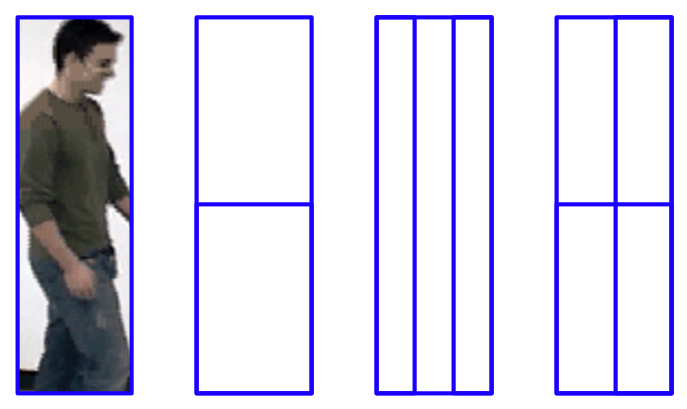
\includegraphics[scale=.4]{img/RectFeatures.jpg}
\caption{Rectangles used for calculating color features.}
\label{fig:rectfeatures}
\end{figure}

The average color intensity for each region of a given rectangle is calculated and constitutes an element of the feature vector for that rectangle. Thus, from left to right, the rectangles in Figure \ref{fig:rectfeatures} have 2, 3, and 4 elements in their feature vectors, respectively. Note that Viola and Jones used a neural network with about a week of training to determine which rectangles worked best for face detection \cite{facedetection}. We simply choose the same rectangles as Yang et al. in \cite{hybrid} and resize them to capture the entire area of the person we wish to track.

For a given region $R_i$, with area $A_i$, we can calculate the average color intensity.

\begin{equation}
(r_i,g_i,b_i) = \sum_{(x,y) \in R_i} (r(x,y), g(x,y), b(x,y))) / A_i
\label{eq:colorregionsum}
\end{equation}

If we let the target color model be ${\bf k}^* = \{ (r_i^*, g_i*, b_i^* \}$ for all regions $i = 1 \dots n$ in the rectangular window, then we can calculate the color similarity between the target color model and a candidate color model ${\bf k}({\bf x}_t)$ for particle ${\bf x}$ at time $t$.

\begin{equation}
\rho({\bf k}^*, {\bf k}({\bf x}_t)) = \left [ \sum^n_{j = 1} (r_i^* - r_i)^2 + (g_i^* - g_i)^2 + (b_i^* - b_i)^2 \right ] ^{1/2}
\label{eq:colorsimilarity}
\end{equation}

Then we can calculate the probability of the candidate matching the target using the following proportionality.

\begin{equation}
p \text{ $\alpha$ exp} (-\rho^2({\bf k}^*, {\bf k}({\bf x}_t)) / \sigma^2)
\label{eq:colorprob}
\end{equation}


\subsection{Integral Image}

Depending on the number and distribution of particles in the system, the same image pixels intensities may be summed multiple times. In order to increase performance, each we convert each frame of the video into an ``integral image", as discussed in \cite{facedetection}. An integral image is the of the same dimensions as the original image, and maintains the same number of color components, but the value of each pixel takes on the value of the summation of all of the pixel intensities to the top and left of it. This is shown in Figure \ref{fig:integralimg}.
 
 \begin{figure}[H]
\centering
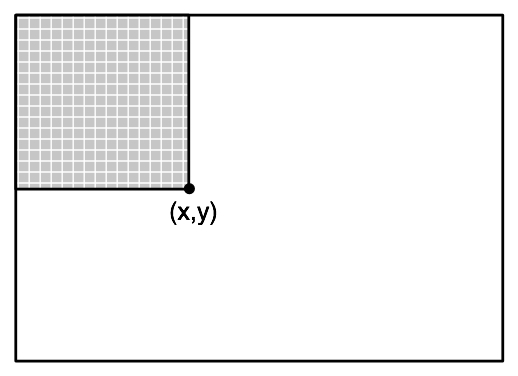
\includegraphics[scale=.4]{img/IntegralImage.jpg}
\caption{Integral image representation. Pixel (x,y) is equal to the summation of the pixel values in the grey region. Based on a figure from \cite{facedetection}.}
\label{fig:integralimg}
\end{figure}

The integral image for each frame is calculated once and then used to calculate the color features for each of the three rectangles for each particle in the system. Using the integral image increases performance because it drastically reduces the total number of particle summations that need to be performed. One can use the integral image to determine the summation of pixel intensities for a given region by adding and subtracting the values of other regions. An example is shown in Figure \ref{fig:integralimguse}.

 \begin{figure}[H]
\centering
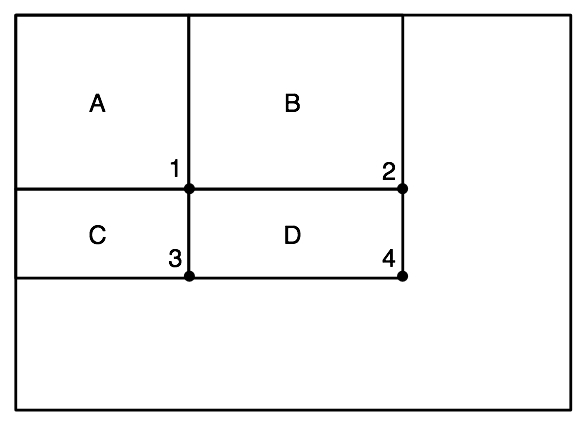
\includegraphics[scale=.4]{img/IntegralImageUse.jpg}
\caption{Example integral image use. Pixel 1 is equal to the summation of all of the pixels in region $A$. Pixel 2 is equal to the summation of all of the pixels in region $A+B$. Pixel 3 is equal to the summation of all of the pixels in region $A+C$. Pixel 4 is equal to the summation of all of the pixels in region $A+B+C+D$. The summation of pixel intensities for region $D$ can be calculated as $4+1-(2+3)$  Based on a figure from \cite{facedetection}.}
\label{fig:integralimguse}
\end{figure}


\subsection{Edge Orientation Histogram Features}
\label{sec:edgehist}

In order to address situations where color information alone is not enough to properly track an object through a scene, we consider edge information. For example, if a person wearing similar colored clothing walks in front of the person being tracked then the current approach may begin to track the new person. To prevent this phenomenon we capture the edge information of the person being tracked. If the person being tracked is standing still, then the edge information for that person will be more vertically oriented than the edge information for the person moving in front of the person being tracked. Comparing edge information is also useful if the color of the person being tracked matches colors in the background of the scene. 

Yang et al. \cite{hybrid} perform edge detection by converting the color image to a greyscale image and then applying the horizontal and vertical Sobel kernels, $K_x$ and $K_y$, respectively.

\begin{equation}
K_x = \left [ \begin{array}{ccc}
+1 & 0 & -1 \\
+2 & 0 & -2 \\
+1 & 0 & -1 \end{array} \right ] 
\label{eq:horzsobel}
\end{equation}

\begin{equation}
K_y = K_x'
\label{eq:vertsobel}
\end{equation}

The horizontal and vertical edge images, $G_x$ and $G_y$, are then computed by convolving ($*$) the Sobel kernels with the greyscale image $I$.

\begin{equation}
G_x(x,y) = K_x * I(x,y)
\label{eq:horzedgeimg}
\end{equation}

\begin{equation}
G_y(x,y) = K_y * I(x,y)
\label{eq:vertedgeimg}
\end{equation}

The strength, $S$, and orientation, $\theta$, of the edges can then be calculated.

\begin{equation}
S(x,y) = \sqrt{G_x^2(x,y) + G_y^2(x,y)}
\label{eq:edgestrength}
\end{equation}

\begin{equation}
\theta = \text{arctan } (G_y(x,y) / G_x(x,y))
\label{eq:edgeorient}
\end{equation}

After removing any values such that $S > 100$  to remove noise, we calculate the normalized horizontal and vertical edge strengths, $g_x$ and $g_y$, for each pixel in the image and use them to partition the edges into 10 bins.

\begin{equation}
g_x(x,y) = G_x(x,y)/S(x,y)
\label{eq:horznormedgestrength}
\end{equation}

\begin{equation}
g_y(x,y) = G_y(x,y)/S(x,y)
\label{eq:vertnormedgestrength}
\end{equation}

We calculate the $g_x$ and $g_y$ image once per frame and separate each into 10 channels where each channel can be thought of as a binary image. For example, if a pixel in $g_x$ channel 5 is assigned a value of 1 it means that pixel was placed in the fifth bin after calculating the histogram for the normalized edge strengths. Similarly to how we calculated average color intensity values for regions within a rectangular window, we can calculate the average number of pixels within a region that have been placed within a certain normalized edge strength histogram bin. To do this we can calculate the integral image for each $g_x$ and $g_y$ channel and then use the arithmetic technique illustrated in Figure \ref{fig:integralimguse}. 

What we end up with is a 10 element feature vector for horizontally oriented edges and a 10 element feature vector for vertically oriented edges. We can then calculate the similarity between a candidate window and the target window using an equation similar to Equation \ref{eq:colorsimilarity} and the calculate the probability of the two being a match using an equation similar to Equation \ref{eq:colorprob}. Yang et al. state that this technique is very similar to the Scale Invariant Feature Transform (SIFT) descriptor.


\subsection{Target Update}

The first stage of our approach calculates the probability of each candidate particle matching the target using the color rectangle features, $p_c$, as described in Section \ref{sec:colorrects}. The particles within the top 5\% $p_c$ are then passed onto the second stage which calculates the probability of each candidate particle matching the target using the edge orientation histogram features, $p_e$, as described in Section \ref{sec:edgehist}. The particles within the top 10\% $p_e$ are considered and the rest are ignored. We multiply the probabilities calculated in these two stages together for each of these particles and choose the particle with the highest resulting combined probability, $p_m = p_c * p_e$, as the new target.

In order to handle slight variations in color (such as changes in lighting conditions) and edge orientation over time, we must update the current target color and edge orientation models. The most naive way would be to simply adopt the newly determined target's color model, $\rho_{c_{n}}$, and edge histogram model, $\rho_{e_{n}}$. This is undesirable because when the person being tracked becomes occluded the current particle may erroneously jump to an undesirable position near the person and capture the background. From that point forward the particles will then attempt to match the background and not the person. To address this issue we maintain the previous color model, $\rho_{c_{t}}$, and edge histogram model, $\rho_{e_{t}}$, and use them to calculate the color model, $\rho_{c_{t+1}}$, and edge histogram model, $\rho_{e_{t+1}}$, that will be matched in the next frame.

\begin{equation}
\rho_{c_{t+1}} = (p_m * \rho_{c_{n}}) + ((1-p_m) * \rho_{c_{t}})
\label{eq:nextcolormodel}
\end{equation}

\begin{equation}
\rho_{e_{t+1}} = (p_m * \rho_{e_{n}}) + ((1-p_m) * \rho_{e_{t}})
\label{eq:nextedgemodel}
\end{equation}

Equation \ref{eq:nextcolormodel} simply calculates the next frame's color model by multiplying the newly determined target's color model times the probability that the new target matches the old target. This value is then added to the product of multiplying the old target's color model times the probability that the new target does not match the old target. Equation \ref{eq:nextedgemodel} does the same for the edge histogram model. In practice this update scheme works well because when the person being tracked becomes occluded $p_m$ is very low, thus almost no alteration is made to the color model or edge model and the particle position does not change. Hence, the tracking window maintains its position over the person being tracked during the occlusion.  



\section{Future Considerations}
\label{sec:future}

Currently the size of the tracking window is constant over the period of time in which a person is being tracked. It would desirable for the window to expand and shrink as the person being tracked moves towards and away from the camera and takes up more and less of the frame area, respectively. We attempted to randomly alter the window width and height for each particle in the particle set slightly to address this. We then observed that for a person walking horizontally across the screen the window would often expand to capture the person's previous position as well as old positions, often increasing in two to three times its original width. Clearly this is undesirable, so the modification was removed from our implementation.



\section{Conclusion}
\label{sec:conclusion}


\newpage
\footnotesize
\bibliographystyle{plain}
\bibliography{project}

\end{document}






